\documentclass[12pt,a4paper]{article}

\usepackage[utf8]{inputenc}
\usepackage[T1]{fontenc}
\usepackage[margin=2.5cm]{geometry}
\usepackage{enumitem}
\usepackage{tabularx}
\usepackage{booktabs}
\usepackage{hyperref}
\usepackage{fancyhdr}
\usepackage{titlesec}
\usepackage{xcolor}
\usepackage{parskip}
\usepackage{tikz}
\usepackage{tcolorbox}

\usetikzlibrary{arrows.meta, positioning}

\definecolor{accent}{HTML}{2C3E50}
\definecolor{muted}{HTML}{7F8C8D}
\definecolor{boxblue}{HTML}{2980B9}
\definecolor{boxgreen}{HTML}{27AE60}
\definecolor{boxred}{HTML}{E74C3C}
\definecolor{boxorange}{HTML}{F39C12}
\definecolor{boxpurple}{HTML}{8E44AD}
\definecolor{lightgray}{HTML}{F4F4F4}

\hypersetup{colorlinks=true, linkcolor=accent, urlcolor=accent}

\pagestyle{fancy}
\fancyhf{}
\fancyhead[L]{\small\color{muted}CONFIDENTIAL}
\fancyhead[R]{\small\color{muted}Howin Technologies}
\fancyfoot[C]{\thepage}
\renewcommand{\headrulewidth}{0.4pt}

\titleformat{\section}{\Large\bfseries}{}{0em}{}
\titleformat{\subsection}{\large\bfseries}{}{0em}{}

\newtcolorbox{hookbox}[1]{
    colback=lightgray,
    colframe=#1,
    boxrule=1.5pt,
    arc=4pt,
    left=8pt, right=8pt, top=6pt, bottom=6pt,
}

\begin{document}

% ── TITLE ──
\begin{center}
    \vspace*{3cm}
    {\LARGE\bfseries AI-Powered Team Operations Platform}\\[0.8cm]
    {\large Internal Proposal}\\[2cm]
    {\color{muted}
    Prepared by: Product \& Engineering\\[0.3cm]
    Date: March 31, 2026\\[0.3cm]
    Classification: Internal --- Confidential}
    \vspace*{3cm}
\end{center}

\newpage
\tableofcontents
\newpage

% ══════════════════════════════════════════════
\section{Executive Summary}

One platform to manage tasks, track work, handle attendance, compute salaries, and give management clear visibility --- powered by AI, with minimal manual effort from anyone.

% ══════════════════════════════════════════════
\section{The Problem}

\begin{hookbox}{boxred}
\textbf{Right now, nobody can answer ``what did the team actually do this week?'' without asking each person individually.}
\end{hookbox}

\textbf{Today's reality:}

\begin{itemize}[nosep]
    \item Tasks live in chat threads, meeting notes, and people's heads --- no structured tracking.
    \item Managers spend hours chasing status updates. Developers forget to update task boards.
    \item Attendance and salary run through myHissab --- a tool our own HR team finds frustrating due to poor UX and negative reviews across the board.
    \item Our developers use AI coding tools (Claude Code, Antigravity, Codex) every day, generating rich activity data that \textbf{goes completely untracked}.
    \item Project health is unknown until deadlines are missed.
    \item Developers who work overtime, weekends, or do manual coding/testing get no credit --- their work is invisible.
\end{itemize}

\begin{center}
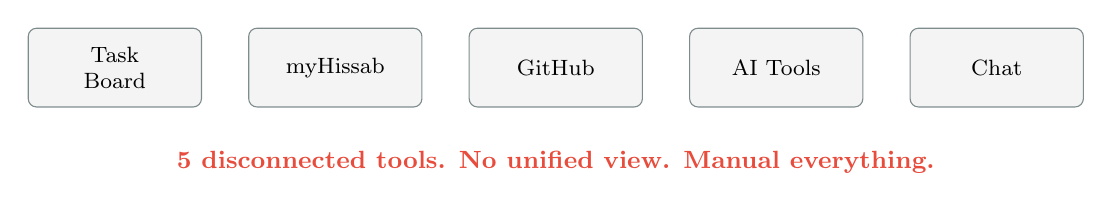
\begin{tikzpicture}[
    tool/.style={rectangle, rounded corners=3pt, minimum width=2.2cm, minimum height=1cm, draw=muted, fill=lightgray, text centered, font=\footnotesize, align=center},
    arr/.style={-, color=muted, thin}
]
    \node[tool] (task) at (0, 0) {Task\\Board};
    \node[tool] (hissab) at (2.8, 0) {myHissab};
    \node[tool] (github) at (5.6, 0) {GitHub};
    \node[tool] (ai) at (8.4, 0) {AI Tools};
    \node[tool] (slack) at (11.2, 0) {Chat};

    \node[font=\small\bfseries\color{boxred}] at (5.6, -1.2) {5 disconnected tools. No unified view. Manual everything.};
\end{tikzpicture}
\end{center}

% ══════════════════════════════════════════════
\section{The Solution}

Replace all of the above with \textbf{one platform} that automatically collects, connects, and reports everything.

\begin{center}
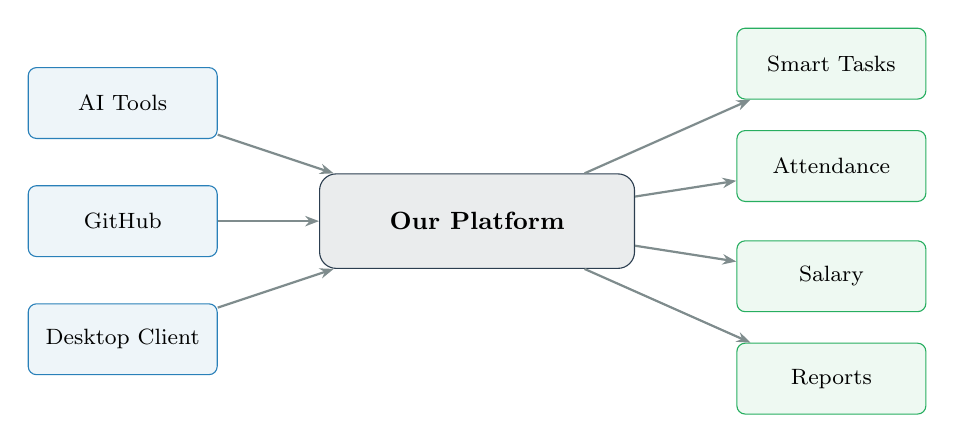
\begin{tikzpicture}[
    input/.style={rectangle, rounded corners=3pt, minimum width=2.4cm, minimum height=0.9cm, draw=boxblue, fill=boxblue!8, text centered, font=\footnotesize, align=center},
    hub/.style={rectangle, rounded corners=6pt, minimum width=4cm, minimum height=1.2cm, draw=accent, fill=accent!10, text centered, font=\small\bfseries},
    output/.style={rectangle, rounded corners=3pt, minimum width=2.4cm, minimum height=0.9cm, draw=boxgreen, fill=boxgreen!8, text centered, font=\footnotesize, align=center},
    arr/.style={-{Stealth[length=5pt]}, thick, color=muted}
]
    % Inputs
    \node[input] (ai) at (-4.5, 1.5) {AI Tools};
    \node[input] (git) at (-4.5, 0) {GitHub};
    \node[input] (desk) at (-4.5, -1.5) {Desktop Client};

    % Hub
    \node[hub] (platform) at (0, 0) {Our Platform};

    % Outputs
    \node[output] (tasks) at (4.5, 2) {Smart Tasks};
    \node[output] (attend) at (4.5, 0.7) {Attendance};
    \node[output] (salary) at (4.5, -0.7) {Salary};
    \node[output] (reports) at (4.5, -2) {Reports};

    \draw[arr] (ai) -- (platform);
    \draw[arr] (git) -- (platform);
    \draw[arr] (desk) -- (platform);
    \draw[arr] (platform) -- (tasks);
    \draw[arr] (platform) -- (attend);
    \draw[arr] (platform) -- (salary);
    \draw[arr] (platform) -- (reports);
\end{tikzpicture}
\end{center}

% ══════════════════════════════════════════════
\newpage
\section{Platform Modules}

% ── MODULE 1 ──
\subsection{1. Task Management}

\begin{hookbox}{boxpurple}
\textbf{PM pastes meeting notes. AI creates the tasks. Developers just work --- the platform tracks progress automatically.}
\end{hookbox}

\begin{itemize}[nosep]
    \item AI generates tasks from meeting notes, requirements, or uploaded documents
    \item Projects with assigned team members and customizable roles
    \item Smart assignee suggestions based on developer skills and current workload
    \item Progress tracked automatically from code activity, AI sessions, and git commits
    \item GitHub Issues sync --- tasks appear in the developer's repo
    \item Human reviews and approves all AI-generated tasks before they go live
\end{itemize}

\begin{center}
\begin{tikzpicture}[
    step/.style={rectangle, rounded corners=3pt, minimum width=2cm, minimum height=1.2cm, draw=boxpurple!60, fill=boxpurple!6, text centered, font=\scriptsize, align=center},
    arr/.style={-{Stealth[length=4pt]}, color=boxpurple!60}
]
    \node[step] (input) at (0, 0) {Meeting\\Notes};
    \node[step] (ai) at (2.8, 0) {AI Creates\\Tasks};
    \node[step] (review) at (5.6, 0) {PM\\Reviews};
    \node[step] (assign) at (8.4, 0) {Smart\\Assignment};
    \node[step] (track) at (11.2, 0) {Auto\\Tracking};

    \draw[arr] (input) -- (ai);
    \draw[arr] (ai) -- (review);
    \draw[arr] (review) -- (assign);
    \draw[arr] (assign) -- (track);
\end{tikzpicture}
\end{center}

% ── MODULE 2 ──
\subsection{2. Attendance \& Salary}

\begin{hookbox}{boxgreen}
\textbf{Replaces myHissab entirely. Attendance is automatic. Salary computation is one click.}
\end{hookbox}

\begin{itemize}[nosep]
    \item Punch in/out via desktop app, web, or mobile (with optional geolocation)
    \item Attendance also derived from real work signals --- git commits, AI sessions, file changes
    \item Work hours calculated from \textbf{actual output}, not just clock time
    \item Leave management: request, approve, track balances (casual, sick, vacation)
    \item Monthly salary auto-computed: base pay, absence deductions, overtime
    \item Exportable reports for payroll --- no more manual spreadsheet work
    \item Overtime automatically detected when someone works outside office hours
\end{itemize}

\begin{center}
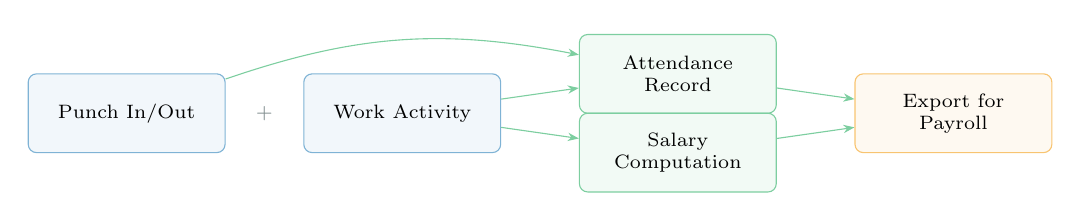
\begin{tikzpicture}[
    box/.style={rectangle, rounded corners=3pt, minimum width=2.5cm, minimum height=1cm, text centered, font=\scriptsize, align=center},
    arr/.style={-{Stealth[length=4pt]}, color=boxgreen!60}
]
    \node[box, draw=boxblue!60, fill=boxblue!6] (punch) at (0, 0) {Punch In/Out};
    \node[box, draw=boxblue!60, fill=boxblue!6] (activity) at (3.5, 0) {Work Activity};

    \node[font=\scriptsize\color{muted}] at (1.75, 0) {+};

    \node[box, draw=boxgreen!60, fill=boxgreen!6] (attend) at (7, 0.5) {Attendance\\Record};
    \node[box, draw=boxgreen!60, fill=boxgreen!6] (salary) at (7, -0.5) {Salary\\Computation};

    \node[box, draw=boxorange!60, fill=boxorange!6] (export) at (10.5, 0) {Export for\\Payroll};

    \draw[arr] (activity) -- (attend);
    \draw[arr] (activity) -- (salary);
    \draw[arr] (punch) edge[bend left=15] (attend);
    \draw[arr] (attend) -- (export);
    \draw[arr] (salary) -- (export);
\end{tikzpicture}
\end{center}

% ── MODULE 3 ──
\subsection{3. Git \& Code Analysis}

\begin{hookbox}{boxblue}
\textbf{``What did this person actually build this week?'' --- answered automatically, without asking anyone.}
\end{hookbox}

\begin{itemize}[nosep]
    \item Connects to GitHub repositories linked to each project
    \item Tracks commits, pull requests, and code reviews per developer
    \item AI summarizes work in plain language: ``Monday: refactored login. Tuesday: built payment API.''
    \item Auto-links commits to tasks via branch names and commit messages
    \item Detects when code was actually written, not just when it was committed
    \item Metrics: commit frequency, languages, PR activity, review turnaround
\end{itemize}

% ── MODULE 4 ──
\subsection{4. Work Activity Tracking}

\begin{hookbox}{boxorange}
\textbf{Tracks all work --- not just AI-assisted work. Manual coding, testing, debugging --- all captured.}
\end{hookbox}

\begin{itemize}[nosep]
    \item File change monitoring in project directories (metadata only --- never reads file contents)
    \item Application context: knows which app is active (for workflow insights, not surveillance)
    \item Auto-discovers project directories from git repos --- zero setup for developers
    \item ``On Watch / Off Watch'' toggle --- personal time is \textbf{never} tracked
    \item Developers can view their own tracking data at any time (full transparency)
\end{itemize}

\textbf{Privacy guarantee:} No screenshots. No keylogging. No file content access. Work is measured by output (code committed, files changed, tasks completed) --- not by how long someone stares at a screen.

% ── MODULE 5 ──
\subsection{5. Desktop Application}

\begin{itemize}[nosep]
    \item System tray app for macOS, Windows, Linux
    \item ``On Watch / Off Watch'' toggle doubles as punch in/out
    \item Shows current task, today's activity, personal stats
    \item Smart reminders during office hours if tracking is off (respects holidays)
    \item Auto punch-out after office hours + configurable buffer
    \item CLI companion for developers who prefer the terminal
\end{itemize}

% ── MODULE 6 ──
\subsection{6. Remote Configuration}

\begin{hookbox}{boxred}
\textbf{Change AI model, permissions, or rate limits for the entire team --- instantly, from one dashboard.}
\end{hookbox}

\begin{itemize}[nosep]
    \item Central control over all AI tool settings
    \item Changes pushed to developer machines in real-time
    \item Full audit trail: who changed what, when, why
    \item Rollback to any previous configuration
    \item Instant cost control when budgets are tight
\end{itemize}

% ── MODULE 7 ──
\subsection{7. Multi-Tool Intelligence}

\begin{itemize}[nosep]
    \item Unified data from Claude Code, Google Antigravity, and Codex
    \item Near-real-time collection from all AI tools
    \item Deduplication --- work isn't double-counted across tools
\end{itemize}

% ── MODULE 8 ──
\subsection{8. Reports \& Project Health}

\begin{hookbox}{boxblue}
\textbf{The daily standup question ``what did you do yesterday?'' is answered before the meeting starts.}
\end{hookbox}

\begin{itemize}[nosep]
    \item \textbf{Daily:} auto-generated standup per developer from actual activity data
    \item \textbf{Weekly:} team summary --- progress, hours, AI usage, highlights
    \item \textbf{Monthly:} executive report --- health, budget, velocity, attendance
    \item \textbf{Project health score} (0--100) per project --- on track / at risk / stalled at a glance
    \item Zero manual effort. Reports write themselves.
\end{itemize}

% ══════════════════════════════════════════════
\newpage
\section{Roles}

\begin{center}
\renewcommand{\arraystretch}{1.4}
\begin{tabularx}{\textwidth}{l X}
    \toprule
    \textbf{Role} & \textbf{Access} \\
    \midrule
    Admin & Full control: users, roles, permissions, config, salary \\
    Project Manager & Tasks, project progress, leave approvals, reports \\
    Developer & Own tasks, own activity, punch in/out, personal stats \\
    Viewer & Read-only dashboards and reports \\
    \bottomrule
\end{tabularx}
\end{center}

Roles are customizable with granular permissions. A person can hold different roles on different projects.

% ══════════════════════════════════════════════
\section{Estimated Impact}

\subsection{Time Savings (10-person team, per month)}

\begin{center}
\renewcommand{\arraystretch}{1.4}
\begin{tabularx}{\textwidth}{X r}
    \toprule
    \textbf{Activity Eliminated / Reduced} & \textbf{Hours Saved} \\
    \midrule
    Meeting notes to task creation (PM) & $\sim$8 hrs \\
    Daily standup preparation (all developers) & $\sim$25 hrs \\
    Manual task status updates & $\sim$15 hrs \\
    Manager status checks \& follow-ups & $\sim$12 hrs \\
    Attendance tracking \& reconciliation (replaces myHissab) & $\sim$10 hrs \\
    Monthly salary processing & $\sim$6 hrs \\
    \midrule
    \textbf{Total} & \textbf{$\sim$76 hrs/month} \\
    \bottomrule
\end{tabularx}
\end{center}

76 hours per month is nearly half a full-time employee's working hours --- redirected from admin overhead to productive work.

\subsection{What Changes for Each Role}

\begin{center}
\renewcommand{\arraystretch}{1.4}
\begin{tabularx}{\textwidth}{l X X}
    \toprule
    \textbf{Role} & \textbf{Before (today)} & \textbf{After (with platform)} \\
    \midrule
    PM & Manually writes tasks from notes, chases updates & Pastes notes, AI does the rest, progress is live \\
    Developer & Forgets to update status, overtime unnoticed & Just works --- system tracks everything \\
    Manager & Asks ``what's the status?'' constantly & Opens dashboard, sees everything \\
    HR & Fights with myHissab monthly & One-click salary export \\
    \bottomrule
\end{tabularx}
\end{center}

\subsection{Other Benefits}

\begin{itemize}[nosep]
    \item \textbf{Better decisions} --- data replaces gut feeling
    \item \textbf{Fair accountability} --- measured by output, not screen time
    \item \textbf{Fewer tools} --- replaces task board, myHissab, time tracker, reporting tools
    \item \textbf{Developer goodwill} --- overtime captured, contributions visible, no micromanagement
    \item \textbf{Cost control} --- instant AI tool spending adjustments from one dashboard
\end{itemize}

% ══════════════════════════════════════════════
\section{Implementation}

Three phases. Each delivers usable functionality on its own.

\begin{center}
\renewcommand{\arraystretch}{1.5}
\begin{tabularx}{\textwidth}{l X}
    \toprule
    \textbf{Phase 1} & Foundation: database, roles \& permissions, desktop client, activity tracking \\
    \textbf{Phase 2} & Core: task management, attendance \& salary, git analysis, GitHub integration \\
    \textbf{Phase 3} & Intelligence: auto reports, project health, remote config, integrations \\
    \bottomrule
\end{tabularx}
\end{center}

% ══════════════════════════════════════════════
\section{Risks}

\begin{center}
\renewcommand{\arraystretch}{1.4}
\begin{tabularx}{\textwidth}{l X}
    \toprule
    \textbf{Risk} & \textbf{Mitigation} \\
    \midrule
    Team resists tracking & Output-based only, no surveillance, full transparency \\
    Scope too large & Phased delivery, each phase self-contained \\
    AI costs & Batch processing, efficient architecture \\
    AI gets it wrong & Human review on all AI suggestions \\
    \bottomrule
\end{tabularx}
\end{center}

% ══════════════════════════════════════════════
\section{Conclusion}

\textbf{Five principles:}

\begin{enumerate}
    \item \textbf{Measure output, not screen time.} Work = code committed, files changed, tasks completed.
    \item \textbf{Automate the mundane.} Standups, status updates, attendance, salary --- all automated.
    \item \textbf{AI assists, humans decide.} Every AI suggestion goes through human review.
    \item \textbf{One platform, complete visibility.} Tasks, time, code, analytics --- one login.
    \item \textbf{Respect privacy.} No screenshots, no keylogging. Track output, not behavior.
\end{enumerate}

\vspace{1cm}
\begin{center}
\textit{We're not building a monitoring tool.\\We're building an operations platform that makes every team member more effective.}
\end{center}

\vfill
\begin{center}
\small\color{muted}
Prepared by Product \& Engineering --- March 2026\\
For internal review only. All estimates are subject to refinement.
\end{center}

\end{document}
